El ambiente radiactivo atmosférico se debe principalmente a la interacción de los rayos cósmicos, compuestos esencialmente de helio, de protones, de electrones y de iones pesados, con los átomos de hidrógeno y de oxígeno presentes en la atmósfera.

Esta interacción da nacimiento a nuevas partículas que pueden ser protones, electrones, neutrónes, iones pesados, piones y/o muones. Esta radiación se crea de dos maneras:  por pérdida de energía por inionisación o  por las reacciones nucleares formando una ``ducha'' \mbox{ }de partículas secundarias. 

Con el avance de la tecnología \textit{Very-Large-Scale Integration} (VLSI) y la utilización de transistores cuyos gravados son muy finos, los circuitos integrados se vuelven sensibles a las partículas que tienen una cantidad de energía menores a los 100MeV ~\cite{taber1995}
~\cite{taber1993single}. Los piones de muy baja energía tienen una actuación insignificante en la perturbación del funcionamiento de circuitos integrados. No es precisamente el caso para los iones pesados y los neutrónes. De hecho, los neutrónes son las partículas predominantes en las alturas aviónicas. Estas partículas no son ionizantes y tienen una energía superiores a los 100 MeV. Estas pueden entrar en colisión con los átomos que constituyen las diferentes capas de los componentes electrónicos generando iones que pueden quebrantar el funcionamiento normal de estos. El flujo normal de neutrónes que provienen del sol están estimado a 36 partículas/$cm^2$/hora ~\cite{standard2001measurement}. En la  figura ~\ref{Alturas} se describen las partículas existentes en la atmósfera en función de la altitud ~\cite{o1971natural} ~\cite{o1978luin}. 



\begin{figure}[H]
	\centering
	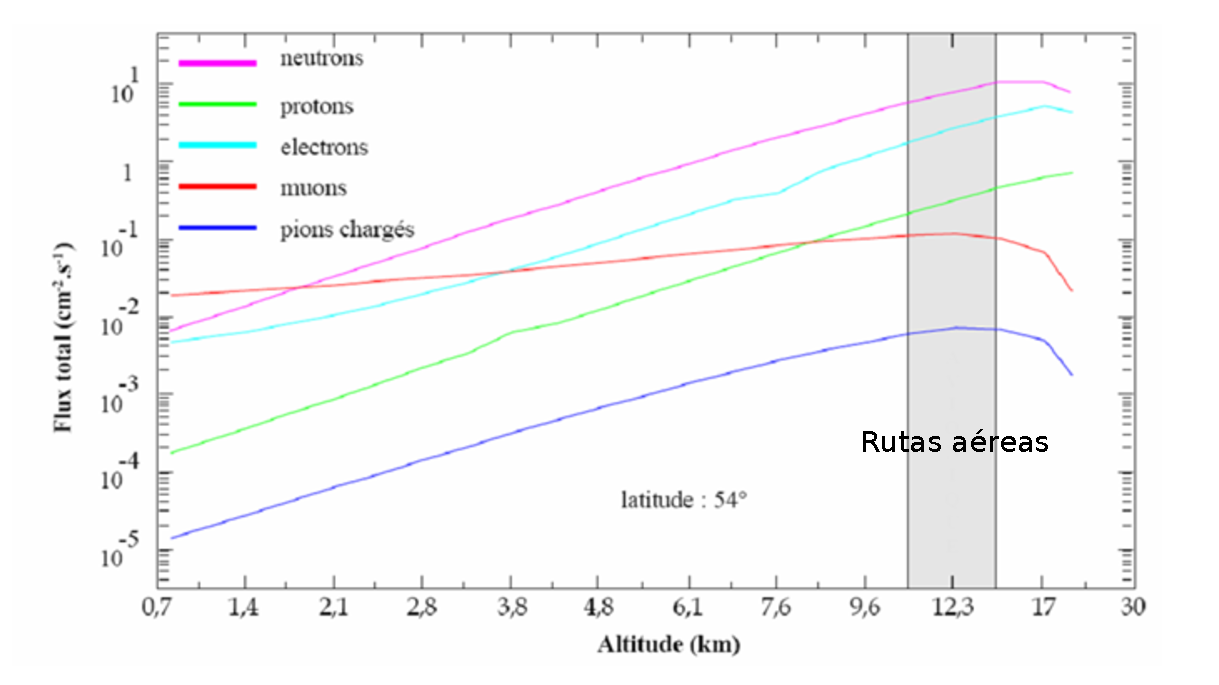
\includegraphics[width=1 \textwidth]{img/Alturas.pdf}
	\caption{Partículas existentes en la atmósfera en función de la altitud   }\cite{mansour2012methodes}
	\label{Alturas}
\end{figure}